\section{Erstellung des Farbschemas}
\label{sec:farbschema}

In diesem Abschnitt wird eine Methode zur Lösung des Teilproblems $f_{scheme}: FGs \to P$ vorgeschlagen. Hierbei werden Farben aus $P$ für die Funktionsgruppen eines Layouts festgelegt, wodurch die Farbgestaltung der Webseite definiert wird. Zur Veranschaulichung wird ein prototypisches Layout für Musikstreaming verwendet. Es enthält die in \autoref{sec:architektur} festgelegten Funktionsgruppen $FGs = $ \{Primär, Sekundär, Akzent, Interaktion, Text (neutral), Hintergrund (neutral)\} . Abbildung \autoref{fig:fgs} hebt die Funktionsgruppen des Layouts separat hervor. Für die Funktionsgruppen \{Primär, Sekundär, Akzent, Interaktion\} werden Farben verwendet, die aus ACoPa resultieren. Für die Funktionsgruppen \{Text (neutral), Hintergrund (neutral)\} wird der Suchraum auf $weiss$ und $schwarz$ beschränkt.

\begin{figure}[]
\centering
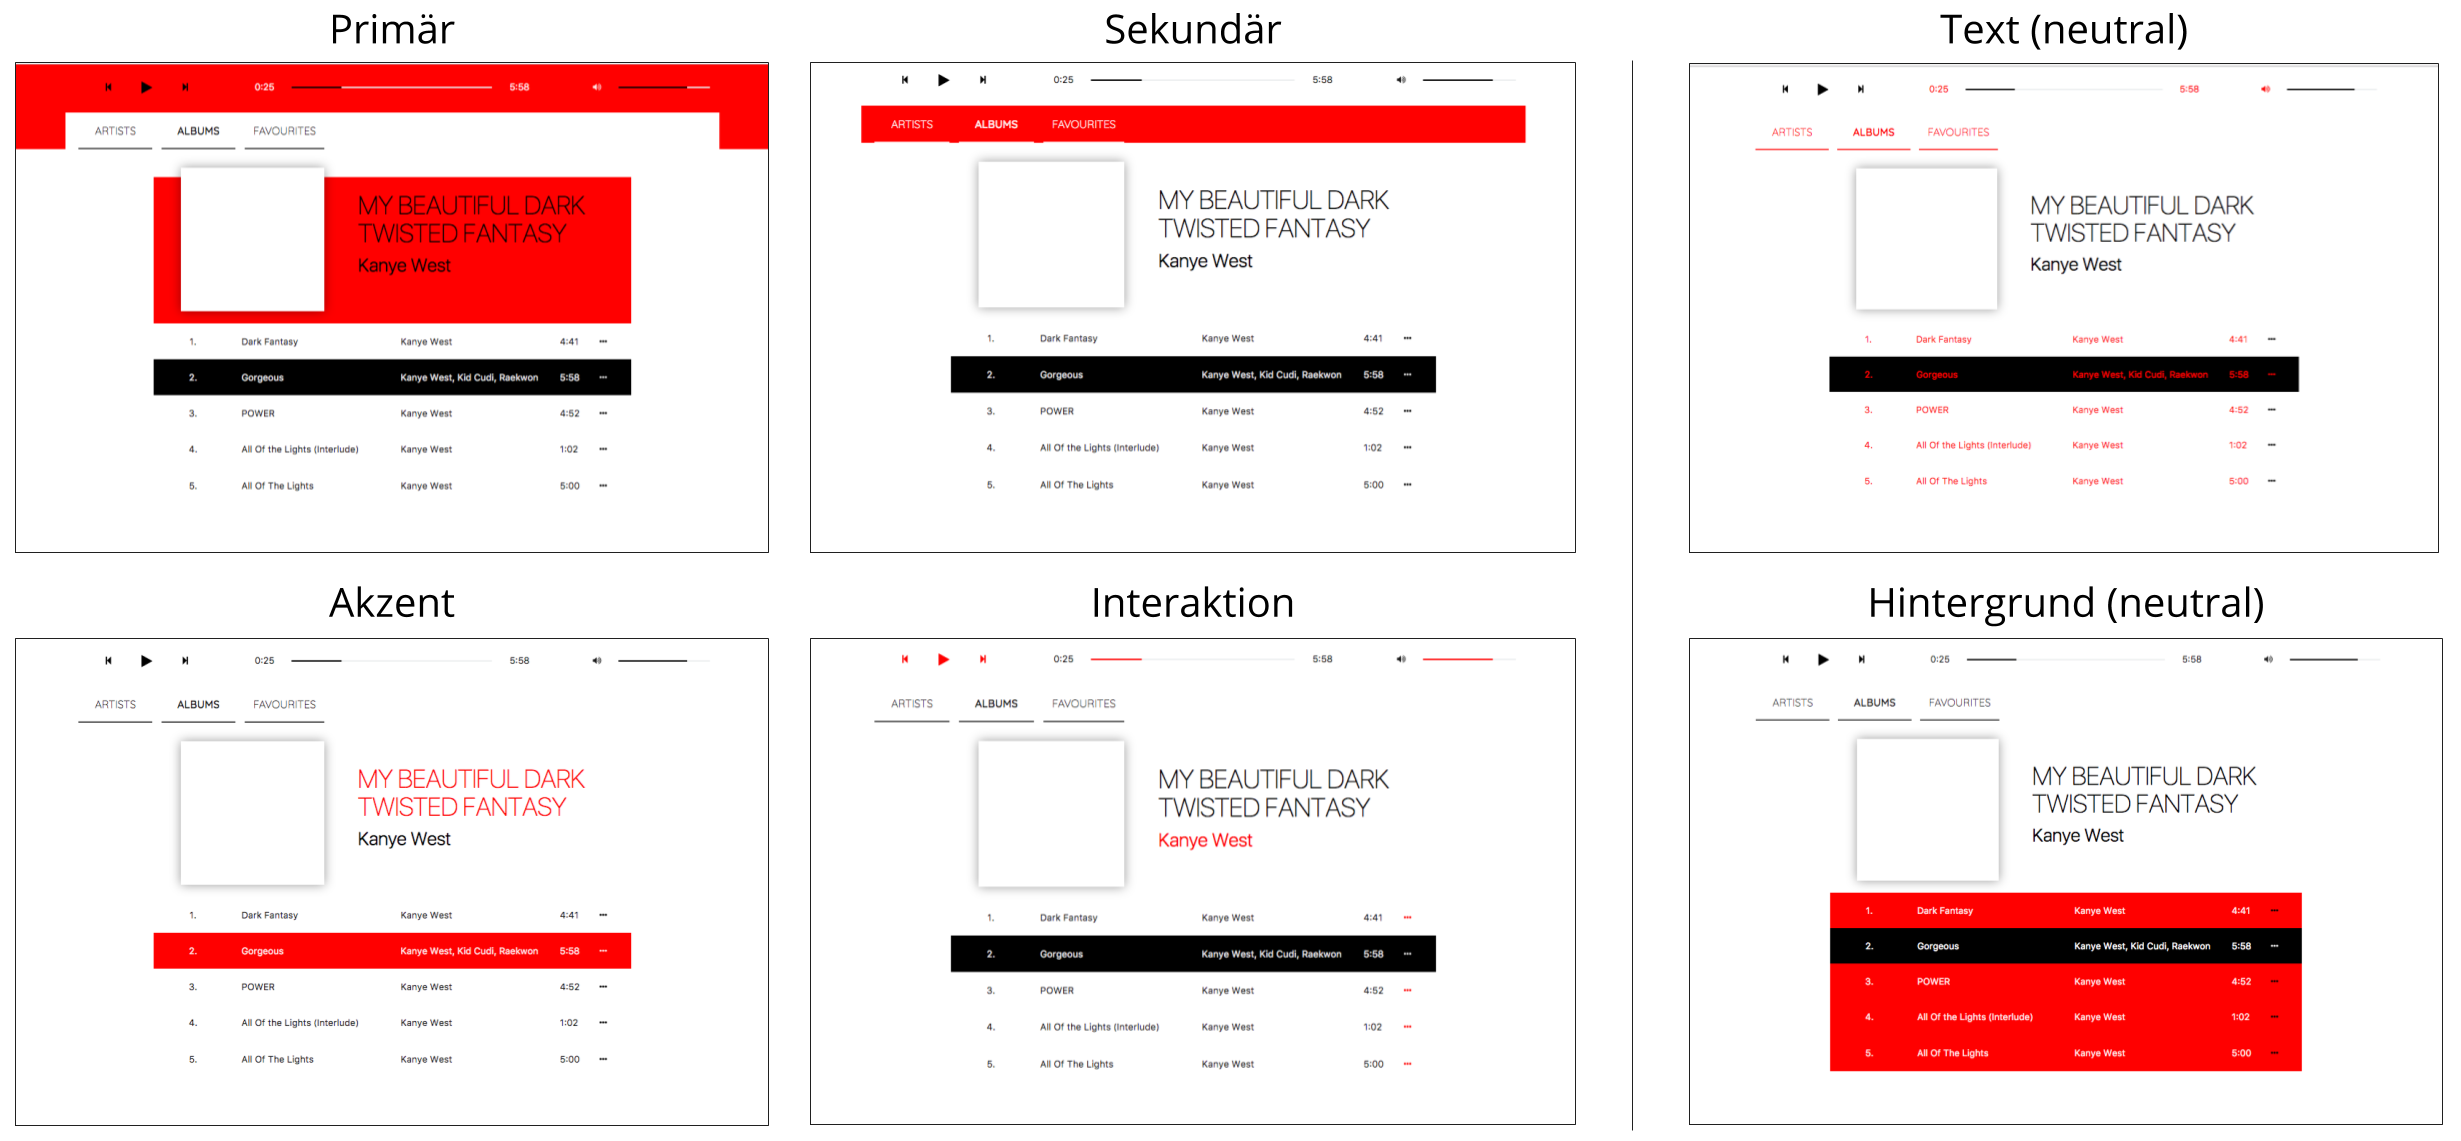
\includegraphics[width=0.95\textwidth]{img/fgs.png}
\caption{Funktionsgruppen des Layouts einer prototypischen Webseite für Musikstreaming. Alle Oberflächenkomponenten, die zur der jeweiligen Funktionsgruppen gehören, sind rot hervorgehoben.}
\label{fig:fgs}
\end{figure}

Als Suchverfahren zur Ermittlung der Abbildung $FGs \to P$ ist ein Suchverfahren zu realisieren. Hierfür werden die Factor Graphs verwendet, die bereits in der Arbeit von \citet{magazines} zur Ermittlung von Farben von Flächen in Mustern erfolgreich eingesetzt wurden. Sie erlauben die Modellierung eines Constraint Graphen, welcher die Faktorisierung einer Wahrscheinlichkeitsverteilung repräsentiert. Zur Implementierung wurde die Bibliothek \emph{Dimple}\footnote{\url{http://dimple.probprog.org/}} für die Programmiersprache Java verwendet.

Der Constraint-Graph besteht aus Knoten und Kanten. Knoten beschreiben Variablen, für die Werte bestimmt werden sollen. Die Variablen repräsentieren $FGs \backslash\{$ Text (neutral)\}. Die Gruppe \{Text (neutral)\} wird ausgelassen, da entsprechend der Erläuterung in \autoref{sec:architektur} die Entscheidung über die Textfarbe auf Layout-Ebene für Blockelemente getroffen wird und nicht Teil des Suchverfahrens ist. Der Wertebereich der Variablen ist eine finite Domain $dom = \{d_0, ..., d_{n+2}\}$, welche der erweiterte Farbpalette $P_\text{neutral} = f_{CPE}(I) \cup \{weiss, schwarz\}$ entsprechen und die Farbwerte um weitere Attribute erweitern. Die lauten:

\begin{itemize}
	\item 
\end{itemize}